\chapter{Design}
In diesem Kapitel geht es darum die Vor- und Nachteile der unterschiedlichen
Bibliotheken anhand eines praktischen Beispieles zu zeigen. Dabei wird
\enquote{gelly-streaming} als Referenz benutzt. Zunächst wird dabei allgemein
der Ablauf des Beispiel beschrieben. Anschließend wir die Architektur der
jeweiligen Umsetzungen beschrieben und schon auftretende Probleme beschrieben.
Abschließend werden mögliche Lösungsstrategien für die Probleme erläutert.

\section{Analyse des Beispieles}
In dem Beispiel geht es darum zu überprüfen, ob ein Graph bipartite ist oder
nicht. Dies bedeutet, ob ein Graph zweifarbig färbbar ist. Um dies für einen
existierenden Graphen zu lösen, gibt es verschiedene Algorithmen. Die allgemeine
Vorgehensweise ist dabei ähnlich.

Am Begin sind alle Knoten ungefärbt. Dann werden zwei Farben gewählt.
Anschließend wird ein Startknoten gewählt und dieser in einer der Farben markiert.
Dann werden die unmarkierten Nachbarknoten in der anderen Farbe markiert. Danach
werden deren unmarkierte Nachbarknoten wieder in der ersten Farbe markiert, usw.
bis alle Knoten makiert sind. Ein Graph ist dann bipartite, wenn alle Knoten so
markiert sind, dass keine benachbarten Knoten die selbe Farbe haben. Diese
Vorgehensweise kann jeder selbst für kleine Graphen selbst durchführen. Je nachdem
welche Informationen über den zu überprüfenden Graphen existieren, kann der Ablauf
auch verkürzt werden. Wenn der Graph nämlich einen Kreis von ungerader Länge
enthällt ist, kann der Graph nie bipartite sein unabhängig vom gewählten
Startknoten. Die Abbildung \ref{fig:bipartite-six-nodes} zeigt einen bipartiten
Graphen mit einen Kreis der Länge sechs. Während dessen die Abbildung \ref{fig:bipartite-five-nodes}
einen nicht bipartiten Graphen zeigt. Denn der Kreis hat eine ungerade Länge und
lässt sich damit nie mit zwei Farben färben egal welcher Startknoten gewählt
wurde. 

\begin{figure}
\centering
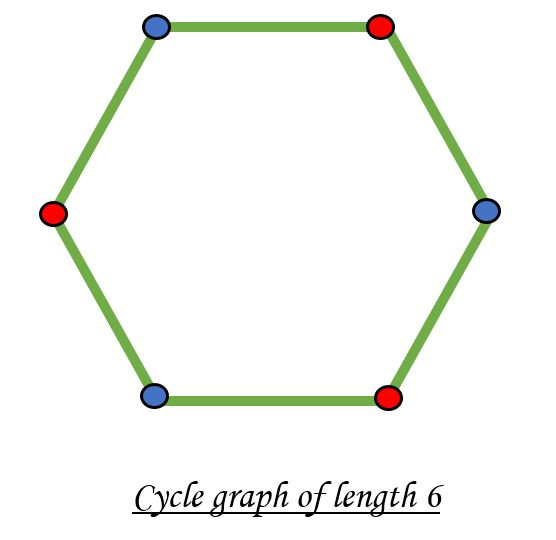
\includegraphics[scale=0.5]{../material/images/bipartite-graph-six-nodes.jpg}
\caption{bipartiter Graph mit Kreis der Länge sechs \cite{GeeksforGeeks2018}}
\label{fig:bipartite-six-nodes}
\end{figure}

\begin{figure}
\centering
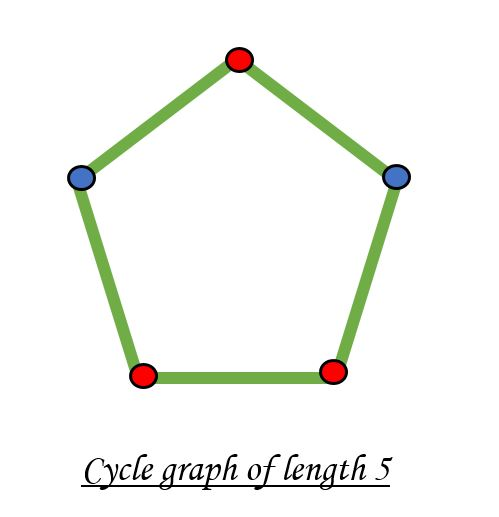
\includegraphics[scale=0.5]{../material/images/bipartite-graph-five-nodes.jpg}
\caption{nicht bipartiter Graph mit Kreis der Länge fünf \cite{GeeksforGeeks2018}}
\label{fig:bipartite-five-nodes}
\end{figure}


Wie läuft das Beispiel nun konkret ab. Zunächst werden die Daten eingelesen. Dies
erfolgt zur Vereinfachung über eine Datei. Dies kann jedoch jederzeit auf eine
alternative Eingabe umgestellt werden zum Beispiel um die Daten von einem
Messaging-System wie Apache Kafka einlesen zu können. Dabei ist zu beachten,
dass alle Bibliotheken, verschiedene Eingabeformate haben, welche in der
Architekturbeschreibung konkret beschrieben werden. Anschließend werden die
Daten an eine beliebige Ausgabe gesendet. Dies ist in unserem Fall einfach die
Konsole. In einer Produktionsumgebung ist dies gerade für Apache Flink
problematisch besonders, wenn es verteilt auf mehrere Rechnern betrieben wird.

\subsection{Architektur}
